\newgeometry{total={210mm,297mm},left=20mm,right=20mm,bindingoffset=5mm, top=25mm,bottom=25mm} 
\begin{partwithabstract}{Results \& Experiments}
    \par{
    The objective of this modelling procedure is to procedure a model that can estimate segmentation masks for the 5 lumbar vertebrae from \acrfull{ct} and \acrfull{mri} scans of human patients, 
    based on point annotation of these 6 classes ($L1$ to $L5$ and 1 background class).
}
\par{
    First, as described in chapter \ref{sec:reference_model}, first a reference is calculated to compare the performance of the weakly supervised models with.
    The reference models are models with the same architecture trained on the same dataset as the weakly supervised models. 
    Contrary to the weakly supervised models, the reference models are trained with full annotation masks instead of point annotated masks. 
}
\par{
    The first step in the modelling procedure based on point annotation masks is the construction of \textit{single-dimension} models.
    Single-dimension indicates that these models investigate the performance of a model that outputs 2D segmentation masks based on 2D input images.
    By slicing the scan volumes along one of three main dimensional axis, a stack of two dimensional images is created together with the point annotation maps extracted from the segmentation masks of these images.
    Chapter \ref{sec:singleDimension} presents the results of several experiments. 
    Models with different loss functions are trained on different point annotation maps where a different number of annotation points is extracted from the full masks.
}
\par{
    the second step in the modelling procedure is the combination of the single-dimension models to estimate pseudo-masks.
    These pseudo masks can finally be used to train a model as if it where true full annotation masks.
    Chapter \ref{sec:combination}, discusses the technique used to combine single-dimension models.
}
\end{partwithabstract}
\restoregeometry



\chapter{Reference model\label{sec:reference_model}}\thispagestyle{empty}
\par{
    As a reference to compare the models trained on weakly-supervised data with, the model performance of a model trained on the same fully supervised data is taken as a reference.
    In this chapter, the results of these fully supervised reference experiments are discussed.
    The metric based on which the experiment results are compared is the inverse class weighted dice score, see equation \ref{eq:weighted_dice} on page \pageref{eq:weighted_dice}.
}
\begin{SCtable}[\sidecaptionrelwidth][h]
 
    % Please add the following required packages to your document preamble:
% \usepackage{multirow}
% Please add the following required packages to your document preamble:
% \usepackage{multirow}

\begin{tabular}{cl|llllll}
    \toprule
    \multicolumn{2}{l|}{\multirow{2}{*}{values in {[}\%{]}}} & \multicolumn{6}{c}{\textbf{Predicted}}                                            \\
    \multicolumn{2}{l|}{}                                    & \textbf{BG} & \textbf{L1} & \textbf{L2} & \textbf{L3} & \textbf{L4} & \textbf{L5} \\ \hline
    \multirow{6}{*}{\textbf{Actual}}      & \textbf{BG}      & 99.9        & 13.2        & 14.5        & 14.2        & 12.9        & 12.1        \\
     & \textbf{L1} & 0 & 86.6 & 2.1  & 0.1  & 0.2  & 0    \\
     & \textbf{L2} & 0 & 0.2  & 83.4 & 0.9  & 0.1  & 0    \\
     & \textbf{L3} & 0 & 0    & 0.1  & 83.9 & 0.4  & 0    \\
     & \textbf{L4} & 0 & 0    & 0    & 1    & 86.1 & 0.7  \\
     & \textbf{L5} & 0 & 0    & 0    & 0    & 0.3  & 87.2 \\ \bottomrule
    \end{tabular}

    \caption{Confusion matrix for the model trained with full label masks (network VGG16-FCN8 and cross-correlation loss), evaluated on the test set.
    The values have been normalized by the total number of voxels predicted in each class.
    The diagonal elements are thus the class precisions: $\mathcal{P}(C = L1 \mid pred = L1) = 0.866$ while $\mathcal{P}(C = L2 \mid pred = L1) = 0.132$.
    \label{tab:full_confusionMatrix}
    }
\end{SCtable}

\section{Experiment results}
\par{
    The fully supervised experiments serve two goals.
    The first is to calculate a reference model performance with which to compare the weakly supervised model results.
    The second is to support hyperparameter choices for the point supervised experiments.
    It is assumed that a network architecture that yields a good, fully supervised model is also a suitable choice to build a weakly supervised model.
    The possible influence of the context slices\footnote{The context slice idea is discussed in detail in chapter \ref{section:twoDplus} on page \pageref{section:twoDplus}.} is also evaluated with these experiments.
}



\par{
    In figure \ref{fig:referenceExperiments}, the results of the reference experiments are shown.
    These results show the network based on VGG16 yields better results than the alternatives based on RESNET50 and U-Net.
    Despite what was hoped for, the context slices do not seem to increase the model performance.
    Remarkably, there is little difference between the models trained with a weighted cross-entropy loss and the non-weighted cross-entropy loss\footnote{
        The weighted cross-entropy loss is defined in chapter \ref{sec:crossentropy} on page \pageref{sec:crossentropy}. 
        The objective of a weighted cross-entropy is to improve the model performance for under-represented classes in an unbalanced dataset by adding a factor inverse proportional to the class prevalence to the cross-entropy loss.
    } when considering the weighted dice score.
    In figure \ref{fig:referenceWeighted}, the model result based on the FCN8 VGG16 model without context slices is compared in detail for the models trained with weighted and the unweighted cross-entropy function.
    Based on these images, some conclusions can be drawn:
    \begin{enumerate}
        \item The prediction of the background class is practically perfect for all datasets.
        \item Other authors \cite{Lessmann2018,Chuang2019} required elaborate evaluation schemes to be able to label the segmented lumbar vertebrae. 
        Due to the larger view ($352 mm \times 352 mm$ vs $180 mm \times 180 mm \times 180 mm$) this model can use by working with 2D slices, it is possible to have all vertebrae in one image.
        The latter proves to allow the model to be trained to identify all five lumbar vertebrae without requiring the evaluation scheme.
        Observe that $\mathcal{P}(C = Li \mid pred = Lj)$ is low for $i\neq j$.
    \end{enumerate}
}
\begin{SCtable}[\sidecaptionrelwidth][h]
    \begin{tabular}{l|llll}
        \toprule
        & \textbf{precision} & \textbf{recall} & \textbf{dice} & \textbf{iou} \\ \hline
        \textbf{Background} & 99.9\%             & 99.7\%          & 99.8\%        & 99.6\%       \\
        \textbf{L1}         & 55.8\%             & 84.0\%          & 67.1\%        & 50.5\%       \\
        \textbf{L2}         & 70.2\%             & 85.2\%          & 77.0\%        & 62.6\%       \\
        \textbf{L3}         & 77.8\%             & 79.9\%          & 78.8\%        & 65.1\%       \\
        \textbf{L4}         & 74.0\%             & 83.2\%          & 78.3\%        & 64.4\%       \\
        \textbf{L5}         & 72.8\%             & 88.2\%          & 79.7\%        & 66.3\%      \\
        \bottomrule
        \end{tabular}
    
        \caption{Per class metric results for the reference model. 
        The performance metrics on the background class are invariably excellent. This is caused by the unbalance in the data.
        Using the inversely weighted dice score gives more weight to the underrepresented classes, which are more of interest.
        \label{tab:full_performanceTable}
        }
    \end{SCtable}
The model trained with an unweighted cross-entropy loss underperforms compared to the model trained with the weighted cross-entropy loss to predict the $L1$ class.
For the other classes, the conclusion based on the inverse weighted dice score holds.

\begin{SCfigure}[][htb]
    \centering
    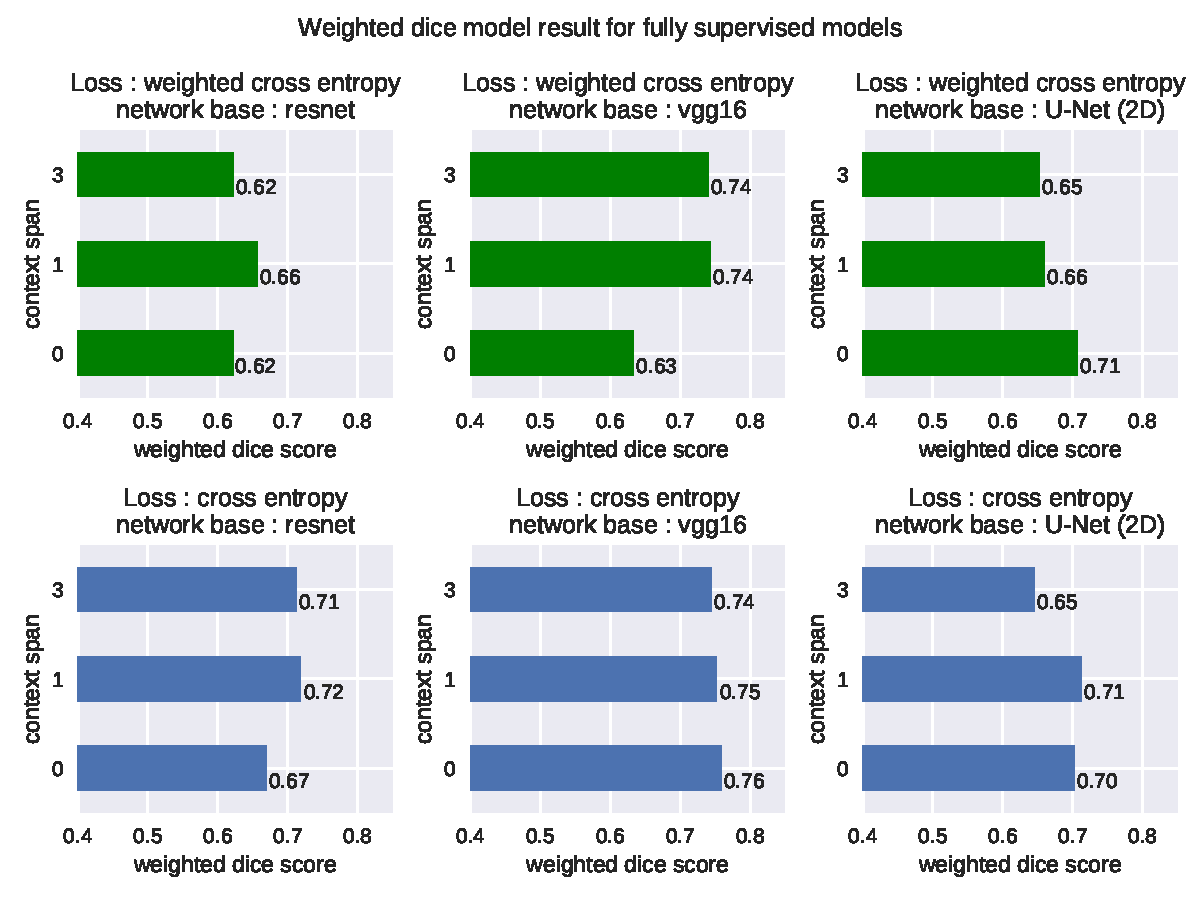
\includegraphics[width=.98\textwidth]{images/FullySupervised.pdf}
    \caption{Results of the fully supervised experiments.
    The indicated model performance metrics are calculated on the test set.
    The columns represent de weighted dice scores for models based on the same network architecture with different loss functions.
    \label{fig:referenceExperiments}}
\end{SCfigure}

\begin{SCfigure}[][htb]
    \centering
    \begin{minipage}{.98\textwidth}
        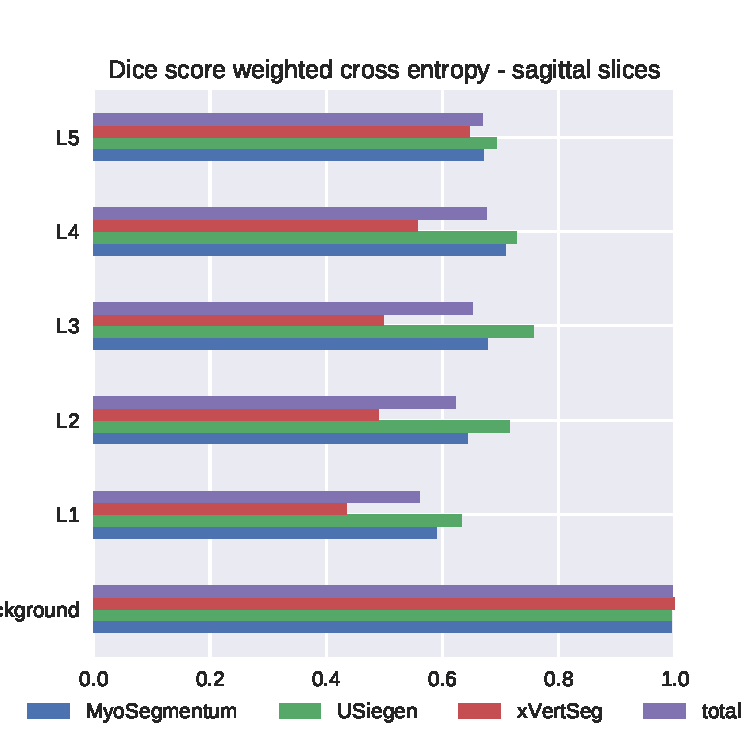
\includegraphics[width=.98\textwidth]{images/full_perClass_perSource_weighted.pdf}
    \end{minipage} 
    \begin{minipage}{0.98\textwidth}
        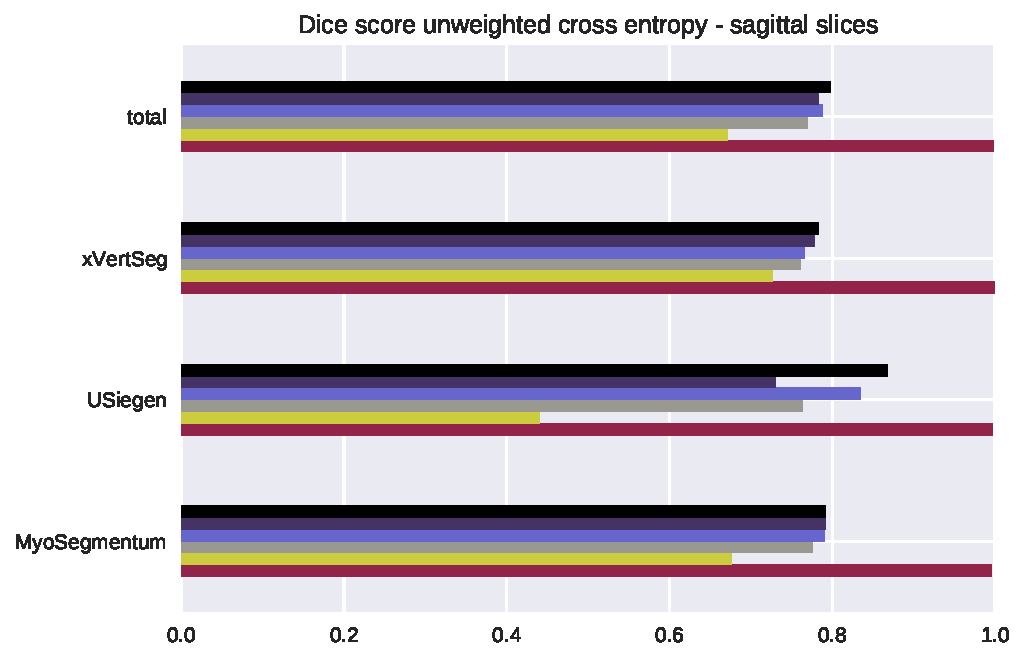
\includegraphics[width=.98\textwidth]{images/full_perClass_perSource_notweighted.pdf}
    \end{minipage}
    \caption{Detailed result for the fully supervised model trained without context slices and with a weighted cross entropy loss function.
    The model trained with the unweighted loss performs better than the result shown in figure \ref{fig:referenceWeighted} for the weighted cross entropy loss function.
    \label{fig:referenceWeighted} 
    }
\end{SCfigure}

\section{Conclusion}
\par{
    Based on the results shown in figure \ref{fig:referenceExperiments}, it was decided to perform the weakly supervised experiments with the model based on VGG16 FCN8 with one context slice.
    The reference performance metric to compare experiments with models trained on weakly supervised data is $\text{Dice}_{wi}=0,76$.
}




\chapter{Single dimension experiments \label{sec:singleDimension}}

\par{
    This chapter discusses the results of several experiments in the construction of single-dimensional models.
    The objective of these experiments is to investigate the influence different model hyperparameters have on the model performance.
    Based on this investigation, the hyperparameters for the single-dimensional models in the final step can be chosen.  
}

\section{Single dimension weakly supervised models}

\par{
    In this section, the results of experiments with different model hyperparameters are compared to each other.
    The point annotation sets are generated from the available full annotation masks for each slice.
    In this work, different datasets were used with different levels of provided annotation. 
    Annotation differences between different datasets are listed in table \ref{tab:datasetReferences} on page \pageref{tab:datasetReferences}.
}
\par{
    For three datasets\footnote{The three datasets for which complete annotation is available are the xVertSeg dataset, the UniSiegen dataset and the MyoSegmentum dataset. Of which the MyoSegmentum dataset is the largest by far.},
    full annotation masks are available, meaning that these scan volumes are labelled with volumes for each of the five lumbar vertebrae.
    For each voxel, the ground truth indicates whether it belongs to a lumbar vertebra and which vertebra.
    For one dataset (PLoS), only semantic segmentation is available. It means that the lumbar vertebrae are indicated as one class but not distinguished. 
    With each voxel in the PLoS dataset, ground truth is associated that indicates if it belongs to a lumbar vertebra. There is no label, however, to indicate which of the lumbar vertebrae this is.
}
\par{
    When a scan is sliced along the craniocaudal axis\footnote{
        The nomenclature of anatomical planes and axis is illustrated in figure \ref{fig:anatomicalPlains} on page \pageref{fig:anatomicalPlains}.
        The craniocaudal axis is the vertical axis when the patient is standing up.} 
    a human can distinguish all 5 lumbar vertebrae (after some practice).
    Therefore, one may hope the single-dimension models trained on sagittal or frontal slices will be able to do the same.
    Even though delineating a vertebra on a transverse slice is possible, identifying which vertebra is presented is challenging for a human.
    Supported by a brief test, it was confirmed that trying to estimate 5 vertebra classes from the transverse slices only provides very confusing results.
    The models trained on the transverse slices only intend to label the slice pixels as either background (0) or vertebra (1), 
    whereas the models trained on the sagittal and frontal slices intend to indicate which of 6 classes\footnote{0 for background, 1 for $L1$, 2 for $L2$, 3 for $L3$, 4 for $L4$ and 5 for $L2$} the pixel belongs to.
}
\par{
    The models trained to segment sagittal and frontal slices were trained on datasets xVertSeg, UniSiegen and MyoSegmenTUM.
    From the available full masks, point annotation labels were extracted.
    The models trained to segment transverse slices\footnote{This segmentation is, as stated not based on distinguishing separate lumbar vertebrae from each other.} 
    are trained on the same three datasets and additionally on the PLoS dataset.    
}
\par{
    The model performance results are compared based on the weighted dice score calculated on the test set.
    This metric is described in chapter \ref{sec:dice} on page \pageref{sec:dice}.
}


\subsection{Evaluation of the model Hyperparameters}

\par{
    To obtain the best model hyperparameters to train the single-dimension models, several tests were conducted to estimate the influence of model components and model hyperparameters\footnote{
        One could argue that the number of annotation points is not a \textit{model} hyperparameter. It is an essential parameter for the \textit{modelling} approach in general.
    } on the model performance.
}

\subsubsection{Weighted vs unweighted point loss performance}

\par{
    Equation \ref{eq:LP} on page \pageref{eq:LP} defines the point loss $\mathcal{L}_P$. 
    In this equation, the factor $w_{\mathcal{Y}_i(\vec{p})}$ indicates a weight that can be assigned to each of the output classes.
    Since data classes can be unbalanced, these weights can help to counter this imbalance.
    In this problem (based on the available datasets), there are about 500 times more background voxels than voxels belonging to a lumbar vertebra.
    By weighing with a factor proportional\footnote{The weighting vector is normalized.} to this ratio, this imbalance can be countered\footnote{
        When full data labels are available, the counts of the voxel types are available for the train set (one should not include the counts of the validation \& test set to avoid data leakage).
        In principle, this information is not necessarily available when only point level annotation is available. In this work, it is considered that (at least an approximation) of the ratios can be available as prior knowledge.
    }. In the unweighted case, $w_{\cdot} = 1$.
}
\par{
    In figure \ref{fig:weighted_vs_unweighted}, the difference between the weighted dice score \& the average dice score on the test set is compared for two models trained on the transverse slices.
    This result shows that the result of the non-weighted segmentation is better than the result of the model trained with weighted loss.
    Contrary to fully supervised models, in the weakly supervised case, the ratio between \textit{labelled} points is not as unbalanced as the ratio between the actual class pixels in the result.
    This explains the weighted point loss performance compared to the unweighted point loss performance.
    An approach that is not tested in this work is to weigh proportional to the inverse of the number of \textit{annotation} points per class instead of weighing proportional to the number of \textit{ground truth} pixels.
}


\begin{SCfigure}[][htb]
    \centering
    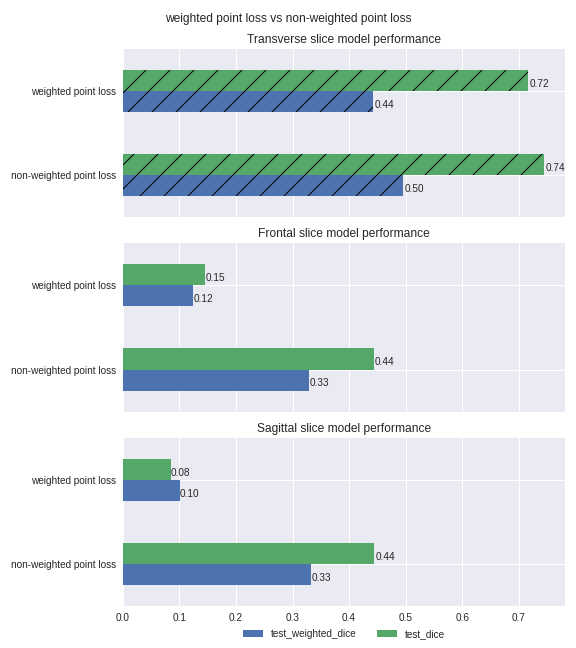
\includegraphics[width=.95\textwidth]{images/weightedvsnonweighted.png}
    \caption{Illustration of the difference in model performance between a weighted point loss function and the unweighted point loss function\label{fig:weighted_vs_unweighted}}
\end{SCfigure}

\subsubsection{Value of the added loss components}
\par{
    In this work, two-loss components were added to the consistency loss published in \cite{Laradji}.
    
    Where \cite{Laradji} is based only on the point loss $\mathcal{L}_P$ and the consistency loss $\mathcal{L}_C$, this work makes use of two extra loss components:
    the prior extend loss $\mathcal{L}_E$ and the separation loss $\mathcal{L}_S$. The four-loss components used in this work are described in more detail in \ref{sec:LossFunctions}.
    Figure \ref{fig:addedLossComponents} shows experimental results validating the positive influence these added loss terms have on the model performance.
}


\begin{SCfigure}[][htb]
    \centering
    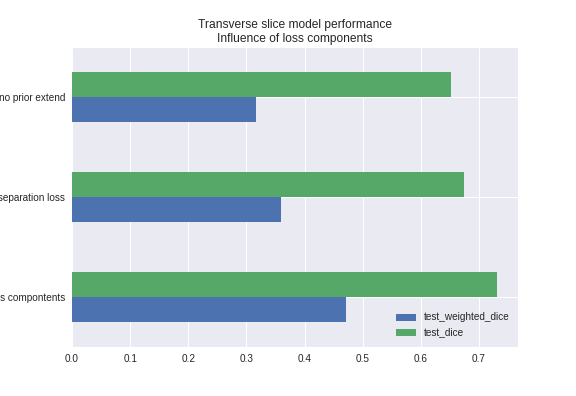
\includegraphics[width=.95\textwidth]{images/TransverseModel_Losscomponents.png}
    \caption{Evaluation of the added value of loss components. \label{fig:addedLossComponents}}
\end{SCfigure}

\subsection{Evolution of the model performance with increased labelling effort}
\par{
    The most basic modelling hyperparameter for a point annotation modelling campaign is the number of labelling points one asks the expert to provide.
    This section presents experimental results to estimate the influence of the number of annotation points on the resulting model performance.
    Intuitively, one would expect the model performance to increase with the number of annotation points provided.
    This hypothesis turns out to be false.
}
\begin{SCfigure}[][htb]
    \centering
    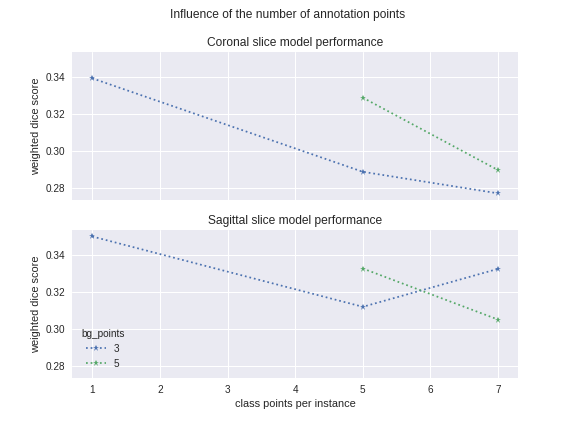
\includegraphics[width=.95\textwidth]{images/BlobPoints_influence.png}
    \caption{Evaluation of the added value of loss components. \label{fig:addedLossComponents}}
\end{SCfigure}
\par{
    Figure \ref{fig:addedLossComponents} shows the weighted dice score actually decreases with more annotation points.
    This is caused by the increased recall of the model. 
    The model becomes very eager to find class points, this causes a lot of background pixels to be wrongly classified as class points.
    The resulting decrease in precision causes the F1 score to decrease.
}
\todo[inline]{Werk verder uit met afbeelding en tabel}



\chapter{Single dimension model combination\label{sec:combination}}

All models are designed for $352 \times 352$ crops of the 2D slices.
The estimation of the slice is obtained by combining the model estimations on all crops taken from this slice.

\section{Volume combination procedure}

Combining the results of three different single dimension models is performed in two steps:
\begin{enumerate}
    \item The resulting classification volumes are first combined with a rule-based method
    \item After this rule-based combination, the resulting segmentation estimation is smoothened with a morphological filter.
\end{enumerate}

\subsection{Rule based result combination}
Three single dimension models are trained:
\begin{description}
    \item[Transverse slices] offer little context to indicate which of the lumbar vertebrae they contain. 
    It does not seem easy even for a human expert to indicate which vertebra is visible on the slice.
    The model trained on these slices is intended only for semantic segmentation.
    Each pixel is inferred only if it represents a vertebra, without distinction between the different lumbar vertebrae. 
    \item[Sagittal \& Coronal slices] do offer the necessary context to distinguish between $L_1$ to $L_5$. 
    The models trained on these slices do indicate the specific lumbar vertebra index. 
\end{description}

Based on the observation that all trained models accurately predict the background, these three models are combined in a straightforward way\footnote{
    The resulting estimations from a model for an input volume is again a three-dimensional volume ($\in \mathbb{N}^3$) with the same dimensions.
}.

\begin{algorithm}[H]
    \SetAlgoLined
    \KwData{
        Results $y_.$ of three models indicating an estimated class for all positions $\vec{p}$ in the volume.
        \begin{itemize} 
            \item Transverse model $y_t \in \mathbb{N}^3: \forall y_t(\vec{p}) \in \{ 0, 1 \}$
            \item Sagittal model $y_s \in \mathbb{N}^3: \forall y_t(\vec{p}) \in \{ 0, 1, 2, 3, 4, 5 \}$ 
            \item Coronal model $y_c \in \mathbb{N}^3: \forall y_t(\vec{p}) \in \{ 0, 1, 2, 3, 4, 5 \}$ 
        \end{itemize}
    }
    \KwResult{Combination of the three model results $y_f$.}
    \For{all $\vec{p}$}{
        \eIf{$y_t[\vec{p}] = 1 \wedge y_s[\vec{p}] = y_c[\vec{p}]$}{
            $y_f[\vec{p}] \leftarrow y_s[\vec{p}]$ \;
        }{
            $y_f[\vec{p}] \leftarrow 0$ \;
        }
    }
   \caption{Rule based combination of model results from three single dimension models}
\end{algorithm}

\todo[inline]{Image illustrating the combination}

\subsection{Morphological smoothing}
After the rule-based combination of estimations from different single dimension models, the result is smoothened with standard morphological filters.
These filters are combinations of the morphological \textit{erosion} and \textit{dilation} operators.
\todo[inline]{How deep should these morphological filters be discussed?}
\begin{itemize}
    \item Possible noise is suppressed by first opening and then closing the volumes.
    \item The estimated volumes are observed to overestimate the extent of the vertebrae. For this reason, an erosion step is performed to decrease the overall extent of the class masks.
\end{itemize}

The procedure mentioned above has two Hyperparameters: the number of iterations for the denoising filters and the number of iterations for the erosion filter.
Both hyperparameters are estimated by calculating the same evaluation metric, the weigh dice score on the validation set, as for the single-dimensional model evaluation. 


\begin{SCfigure}[][htb]
    \centering
    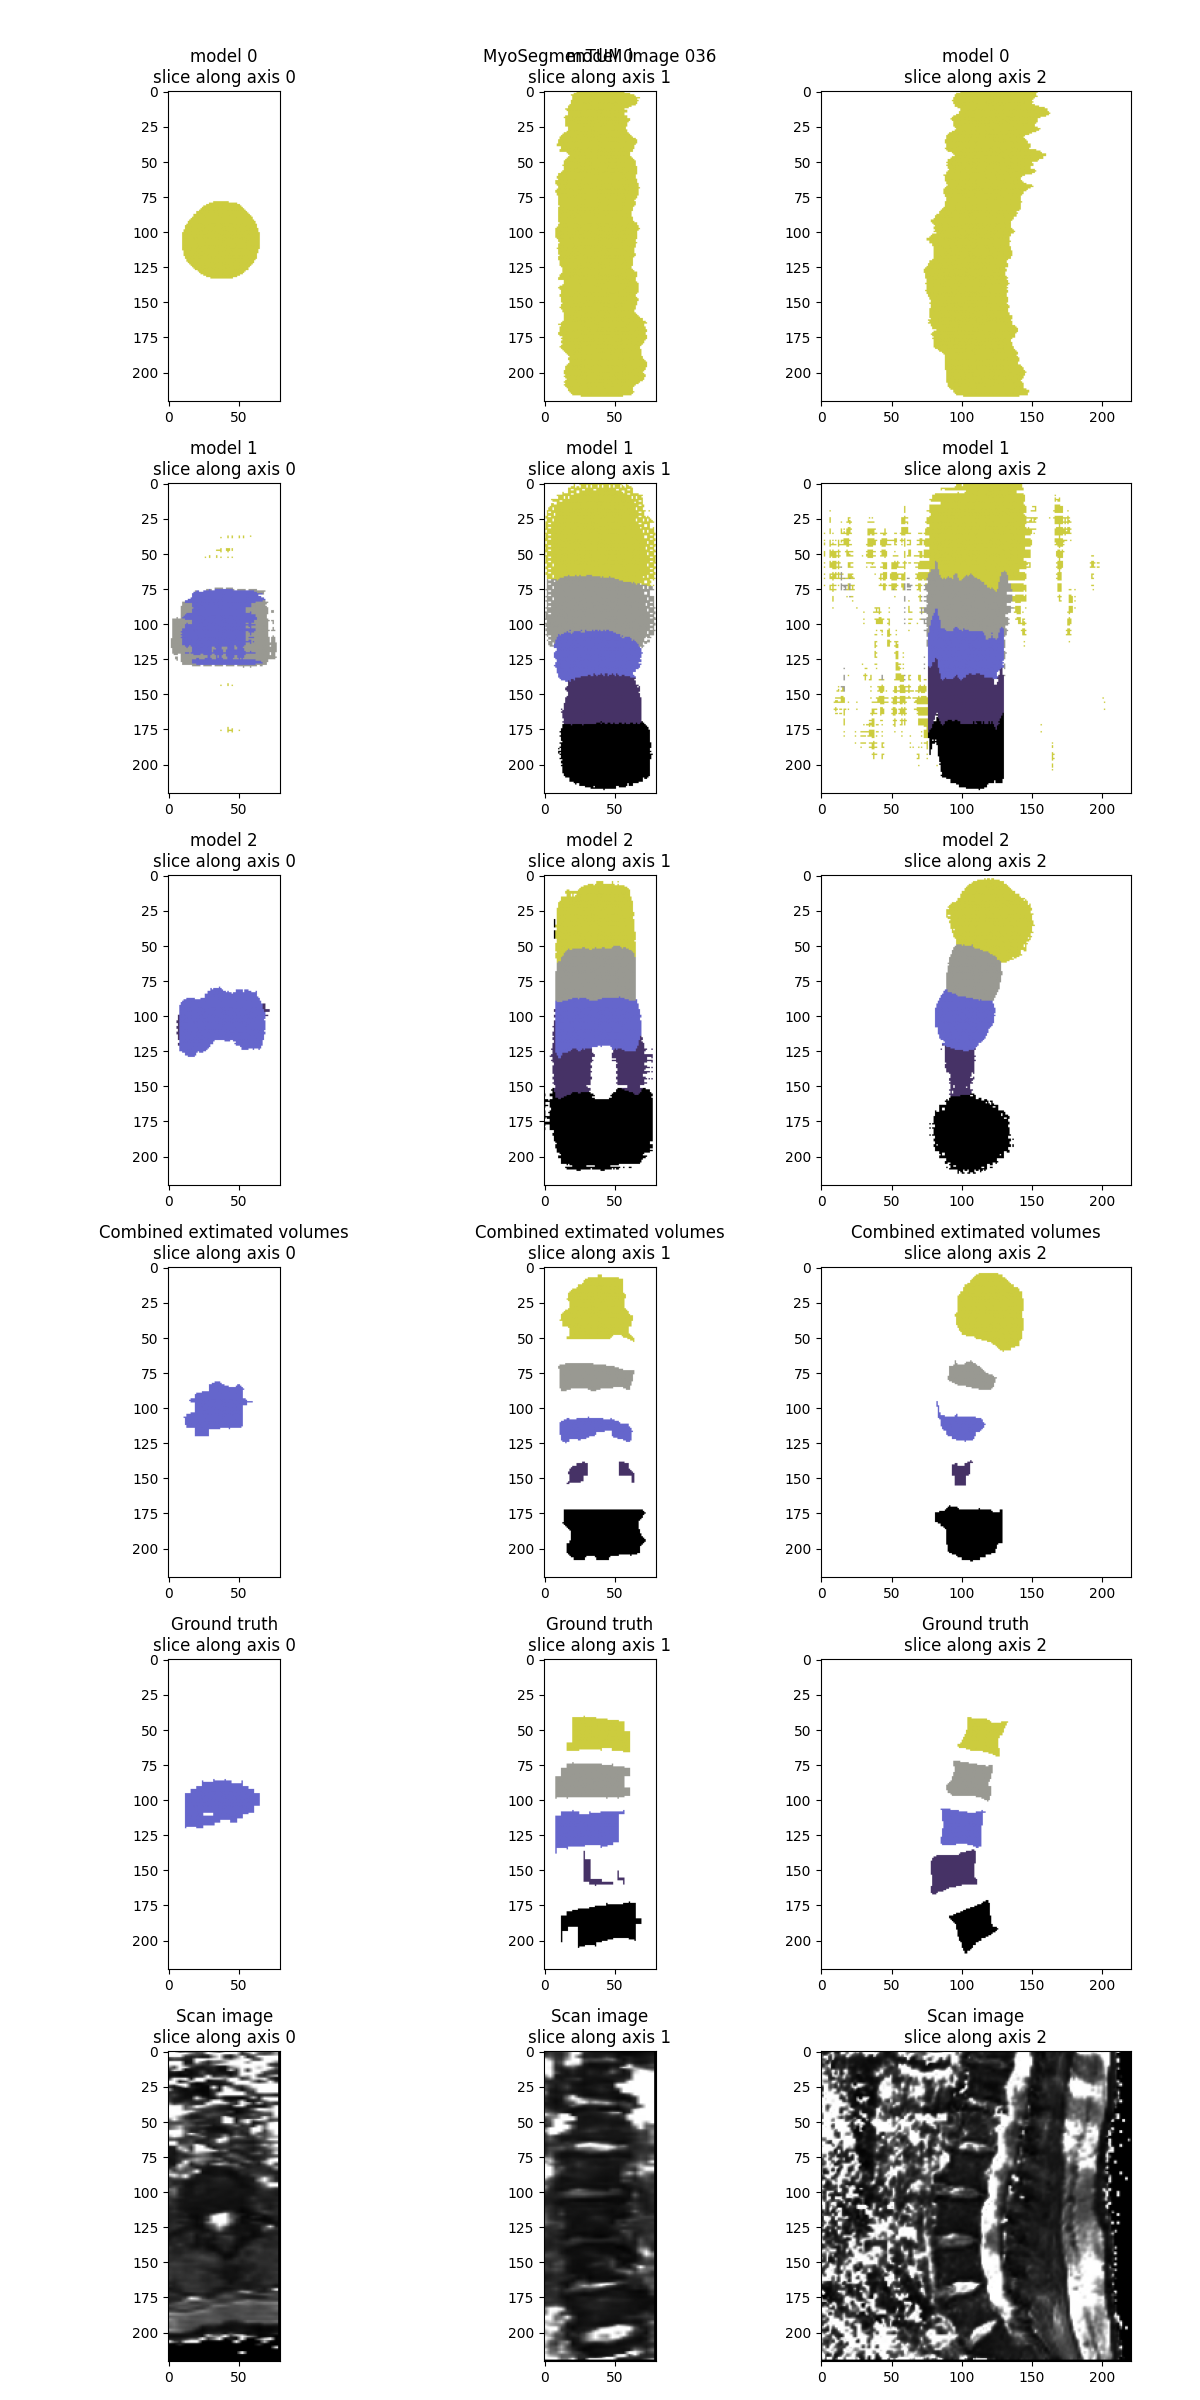
\includegraphics[width=.95\textwidth]{images/morphmask_denoise1_erode1_MyoSegmenTUM_036.png}
    \caption{
        Result of the combination of the three single dimension model results for volume MyoSegmenTUM nr 43.
        The colours indicate the vertebra classes. Only one semantic class is estimated in the first row, illustrating the model trained on transversal slices.
        On the first three rows, slices of the resulting segmentations from the single dimension models are shown. 
        It is clear these masks contain some artefacts and are not always in agreement with each other.
        On the fourth row, the result after mask combination and morphological smoothing is shown. 
        This corresponds more closely to the ground truth mask, shown on the fifth row.
        This final mask, shown on the fourth row, will be used as a pseudo mask to approximate the unknown ground truth mask.
        In the last row, the corresponding images are shown.
    }
\end{SCfigure}

\section{Pseudo mask performance}

\chapter{Pseudo mask training}

Time to evaluate
performance